%!TEX root = ../Thesis.tex
\section{Projektplanung}
\fancyhead[R]{Projektplanung}
\label{instal}

\subsection{Beschreibung des Funktionsumfangs (Florian Rath)}
%%%%%%%%%
%Florian
%%%%%%%%%

Hier den Text einfach hin kopieren.

\subsection{Projektablaufplan (Fabia Schmid)}
%%%%%%%%%
%Fabia
%%%%%%%%%

Als Projektleiterin wählte ich als Vorgehensmodell für die Entwicklung das erweiterte Wasserfallmodell fest. Dafür sprach die klare Struktur des Modelles und der geringe Managementaufwand. Zusätzlich war die Übersichtlichkeit, sowie die leichte Verständlichkeit ein klarer Vorteil. Außerdem sprach für das erweiterte Wasserfallmodell, dass es für kleine Projekte mit festgelegten Umfang ausgelegt und geeignet ist.

Auf diesem Vorgehensmodell basierte die Projektstrukturplanung, die Meilensteinplanung und die Zeitplanung, welche in einem GANTT-Diagramm visualisiert wurde.

\begin{figure}[H]
\centering
\begin{minipage}[t]{1\textwidth} % Breite, z.B. 1\textwidth		
\caption{Projektstrukturplan} % Überschrift
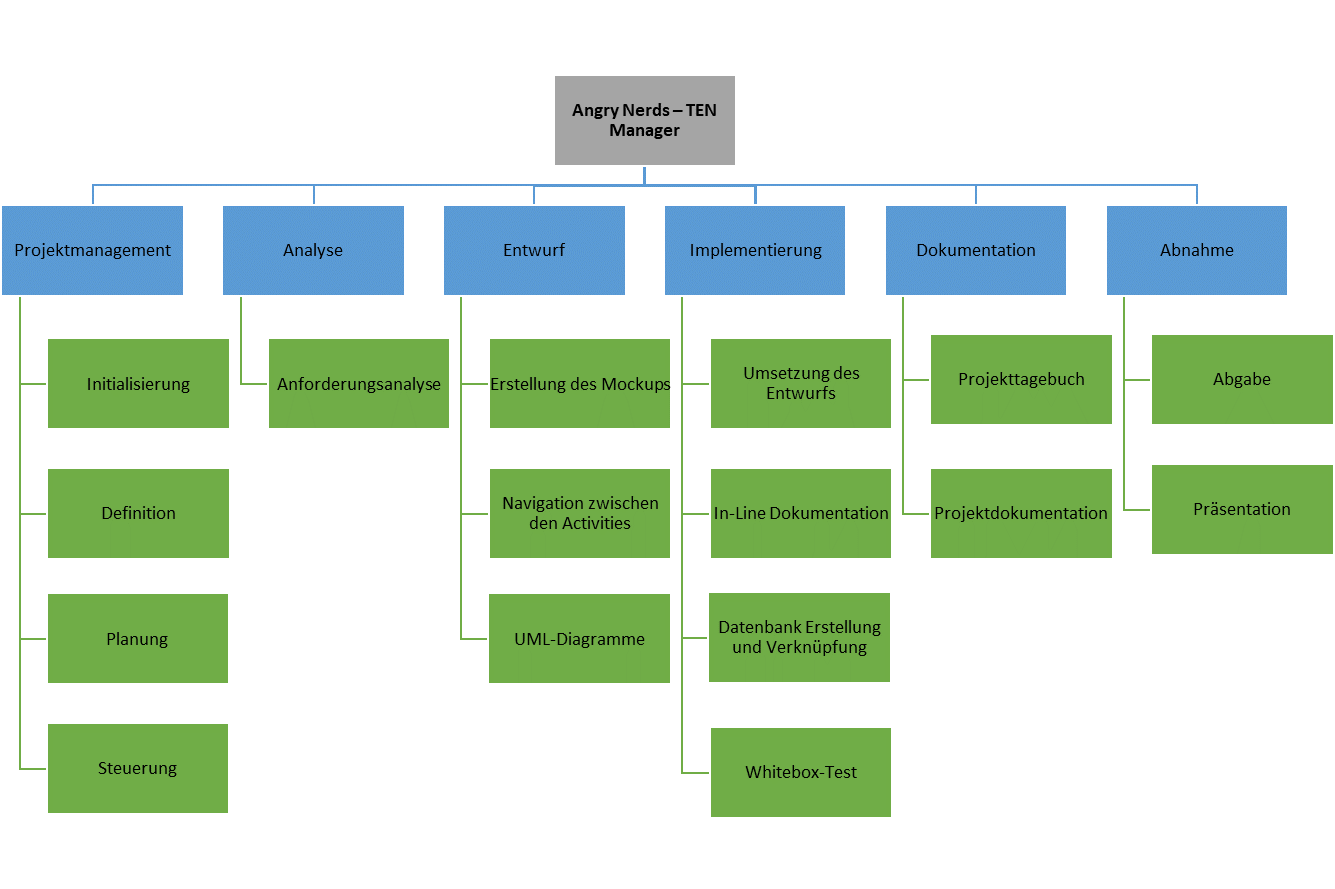
\includegraphics[width=1\textwidth]{img/Projektstrukturplan}\\ % Pfad
\source{Erstellt von Fabia Schmid} % Quelle
\end{minipage}
\end{figure}

\begin{figure}[H]
\centering
\begin{minipage}[t]{1\textwidth} % Breite, z.B. 1\textwidth		
\caption{Meilensteinplan} % Überschrift

\includegraphics[width=1\textwidth]{img/fhdw}\\ % Pfad
\source{Erstellt von Fabia Schmid} % Quelle
\end{minipage}
\end{figure}

\begin{figure}[H]
\centering
\begin{minipage}[t]{1\textwidth} % Breite, z.B. 1\textwidth		
\caption{GANTT-Diagramm} % Überschrift
\includegraphics[width=1\textwidth]{img/GANTT}\\ % Pfad
\source{Erstellt von Fabia Schmid} % Quelle
\end{minipage}
\end{figure}

\begin{figure}[H]
\centering
\begin{minipage}[t]{1\textwidth} % Breite, z.B. 1\textwidth		
\caption{Geplante Aufgabenverteilung} % Überschrift

\includegraphics[width=1\textwidth]{img/fhdw}\\ % Pfad
\source{Erstellt von Fabia Schmid} % Quelle
\end{minipage}
\end{figure}

\newpage
\subsection{Planung der Software}
\subsubsection{Planung des Mock-Ups (Robin Menzel)}
%%%%%%%%%
%Robin
%%%%%%%%%
\begin{figure}[H]
	\subsection*{Übersicht}
	\centering
	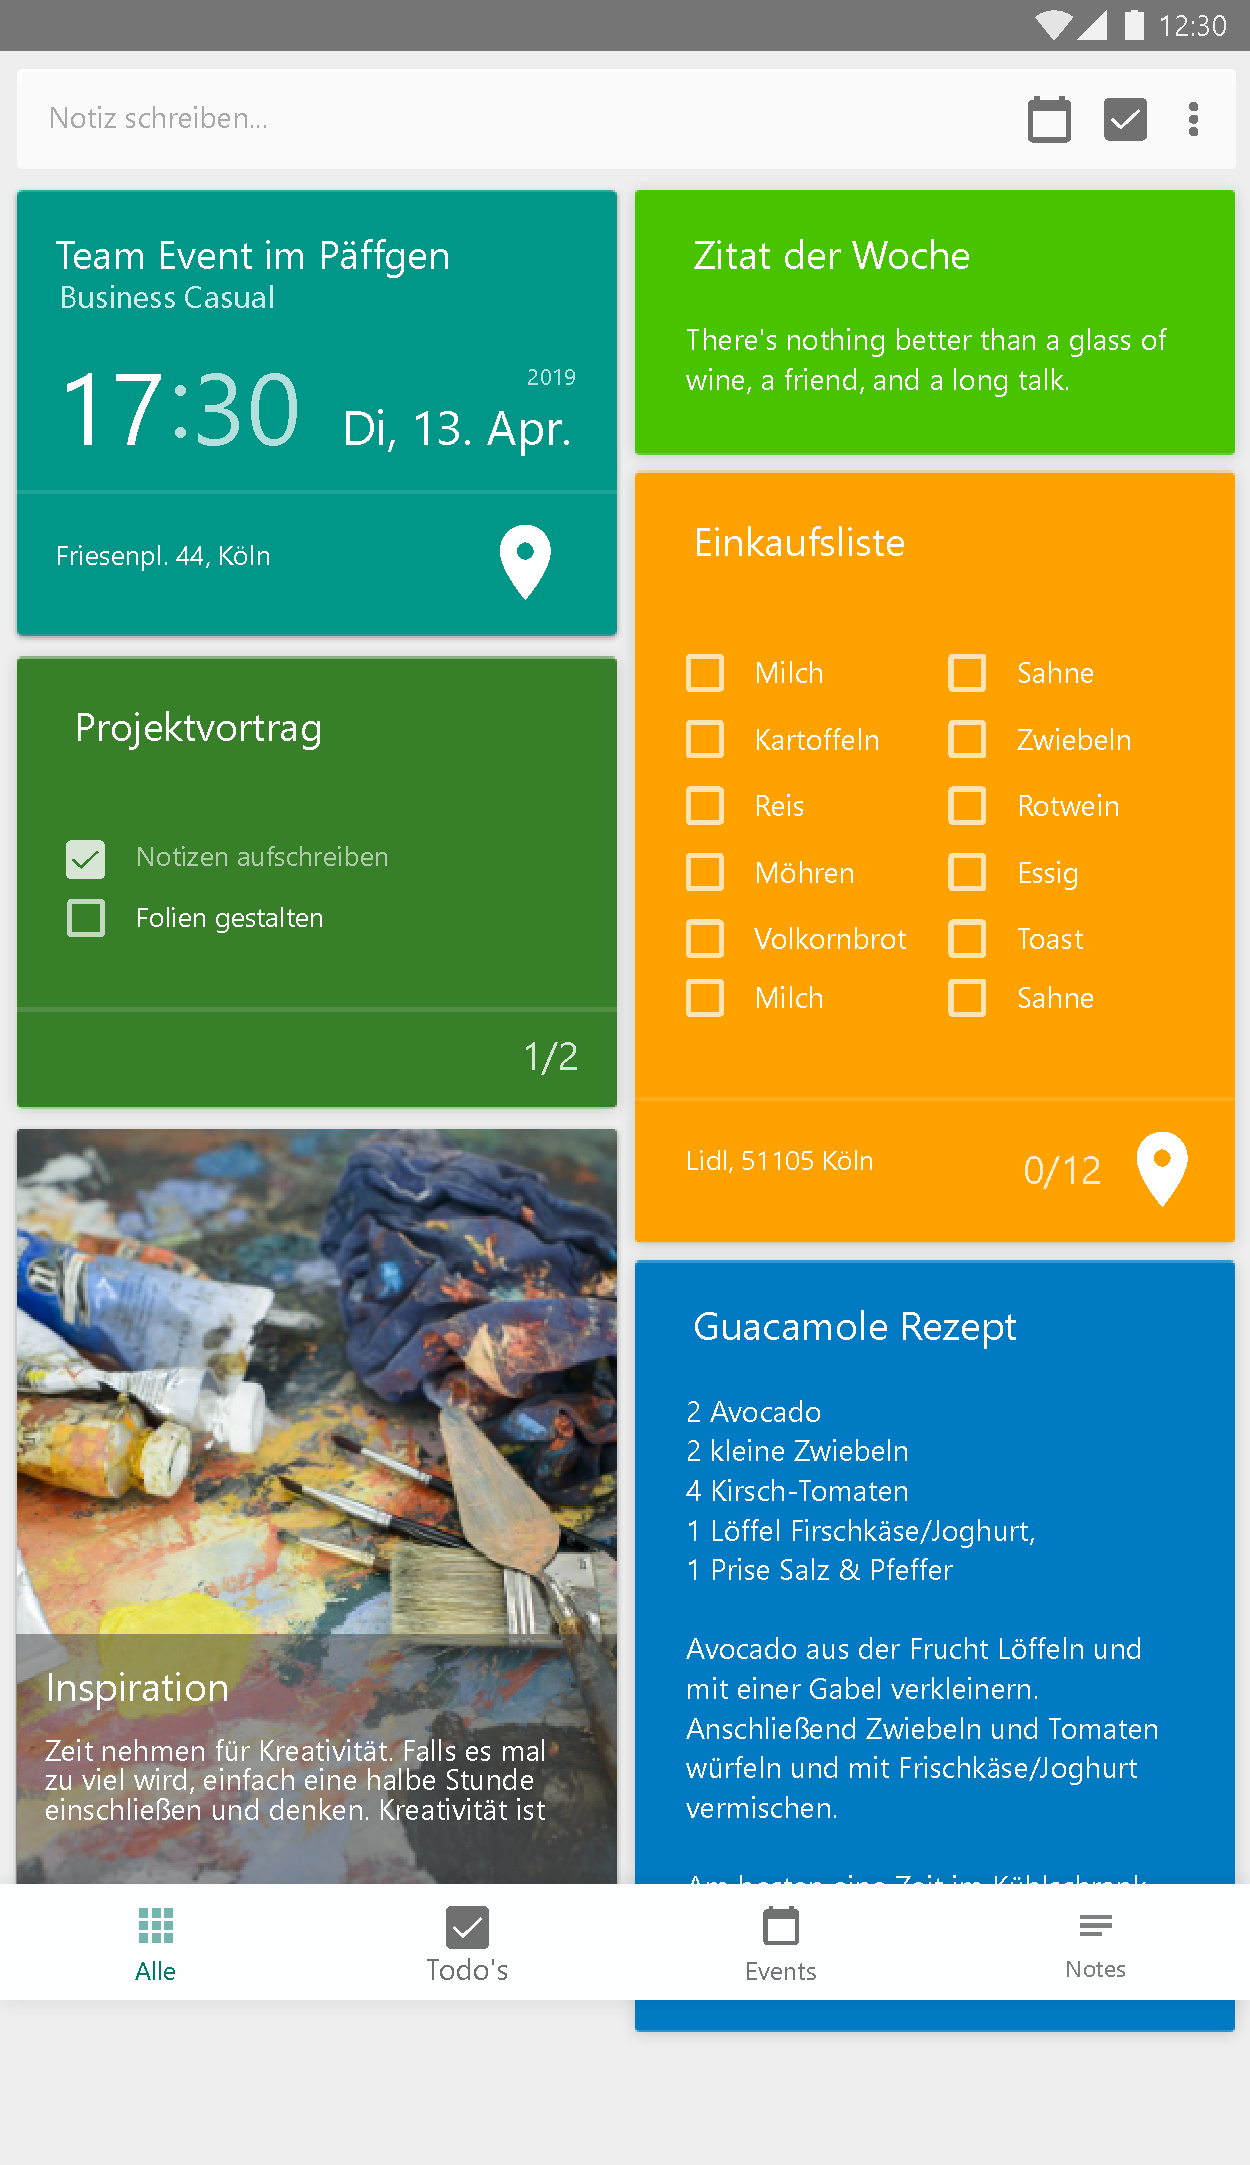
\includegraphics[width=8cm]{img/OverviewActivity.pdf}
	\caption{Mockups - Übersicht über alle TENs}
	\label{img:OverviewActivity}
\end{figure}

\begin{figure}[H]
	\subsection*{Event Activity - Unsere Events}
	\centering
	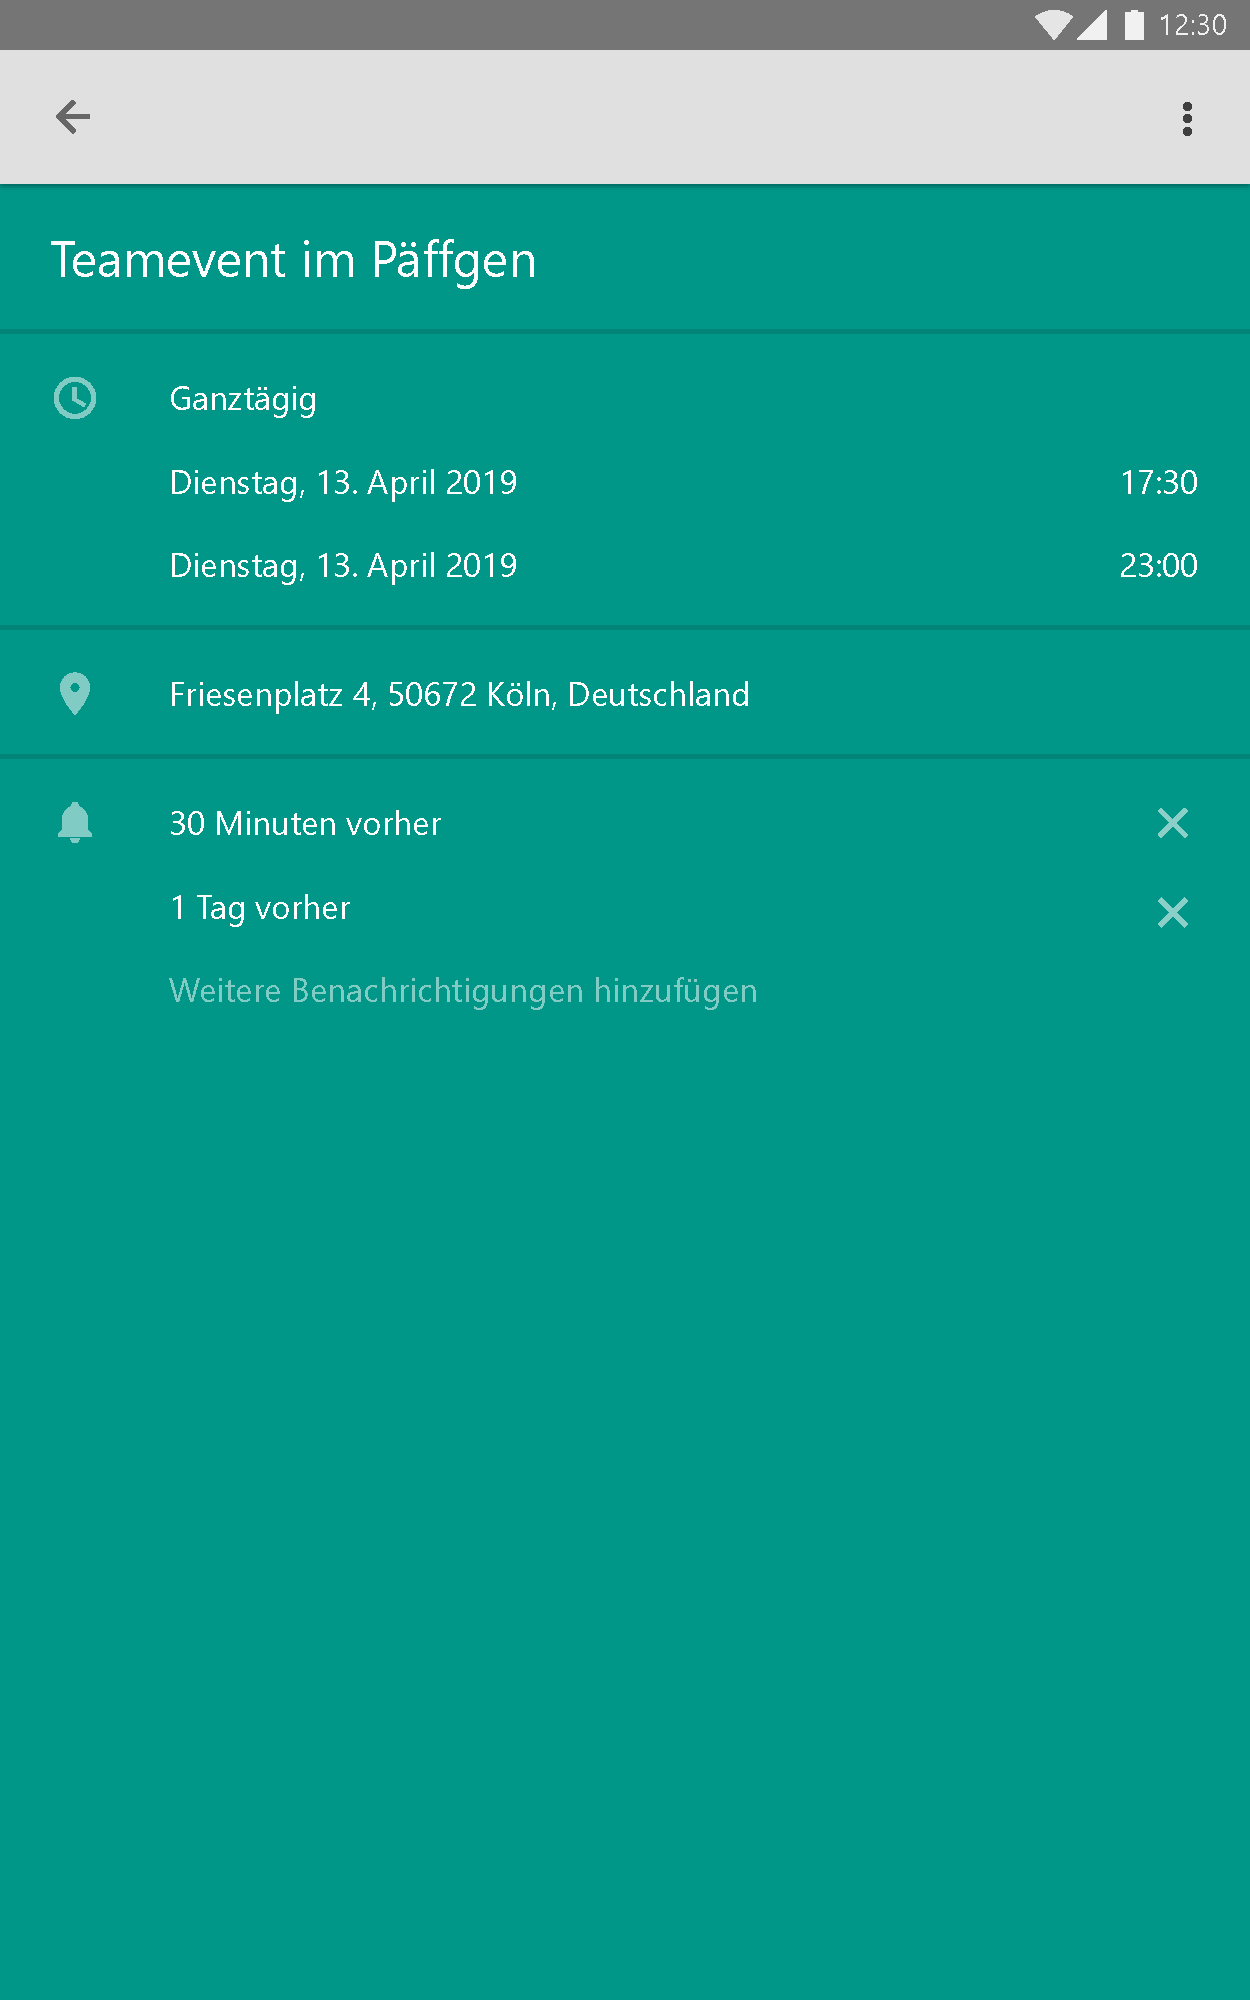
\includegraphics[width=7.25cm]{img/EventActivity.pdf}
	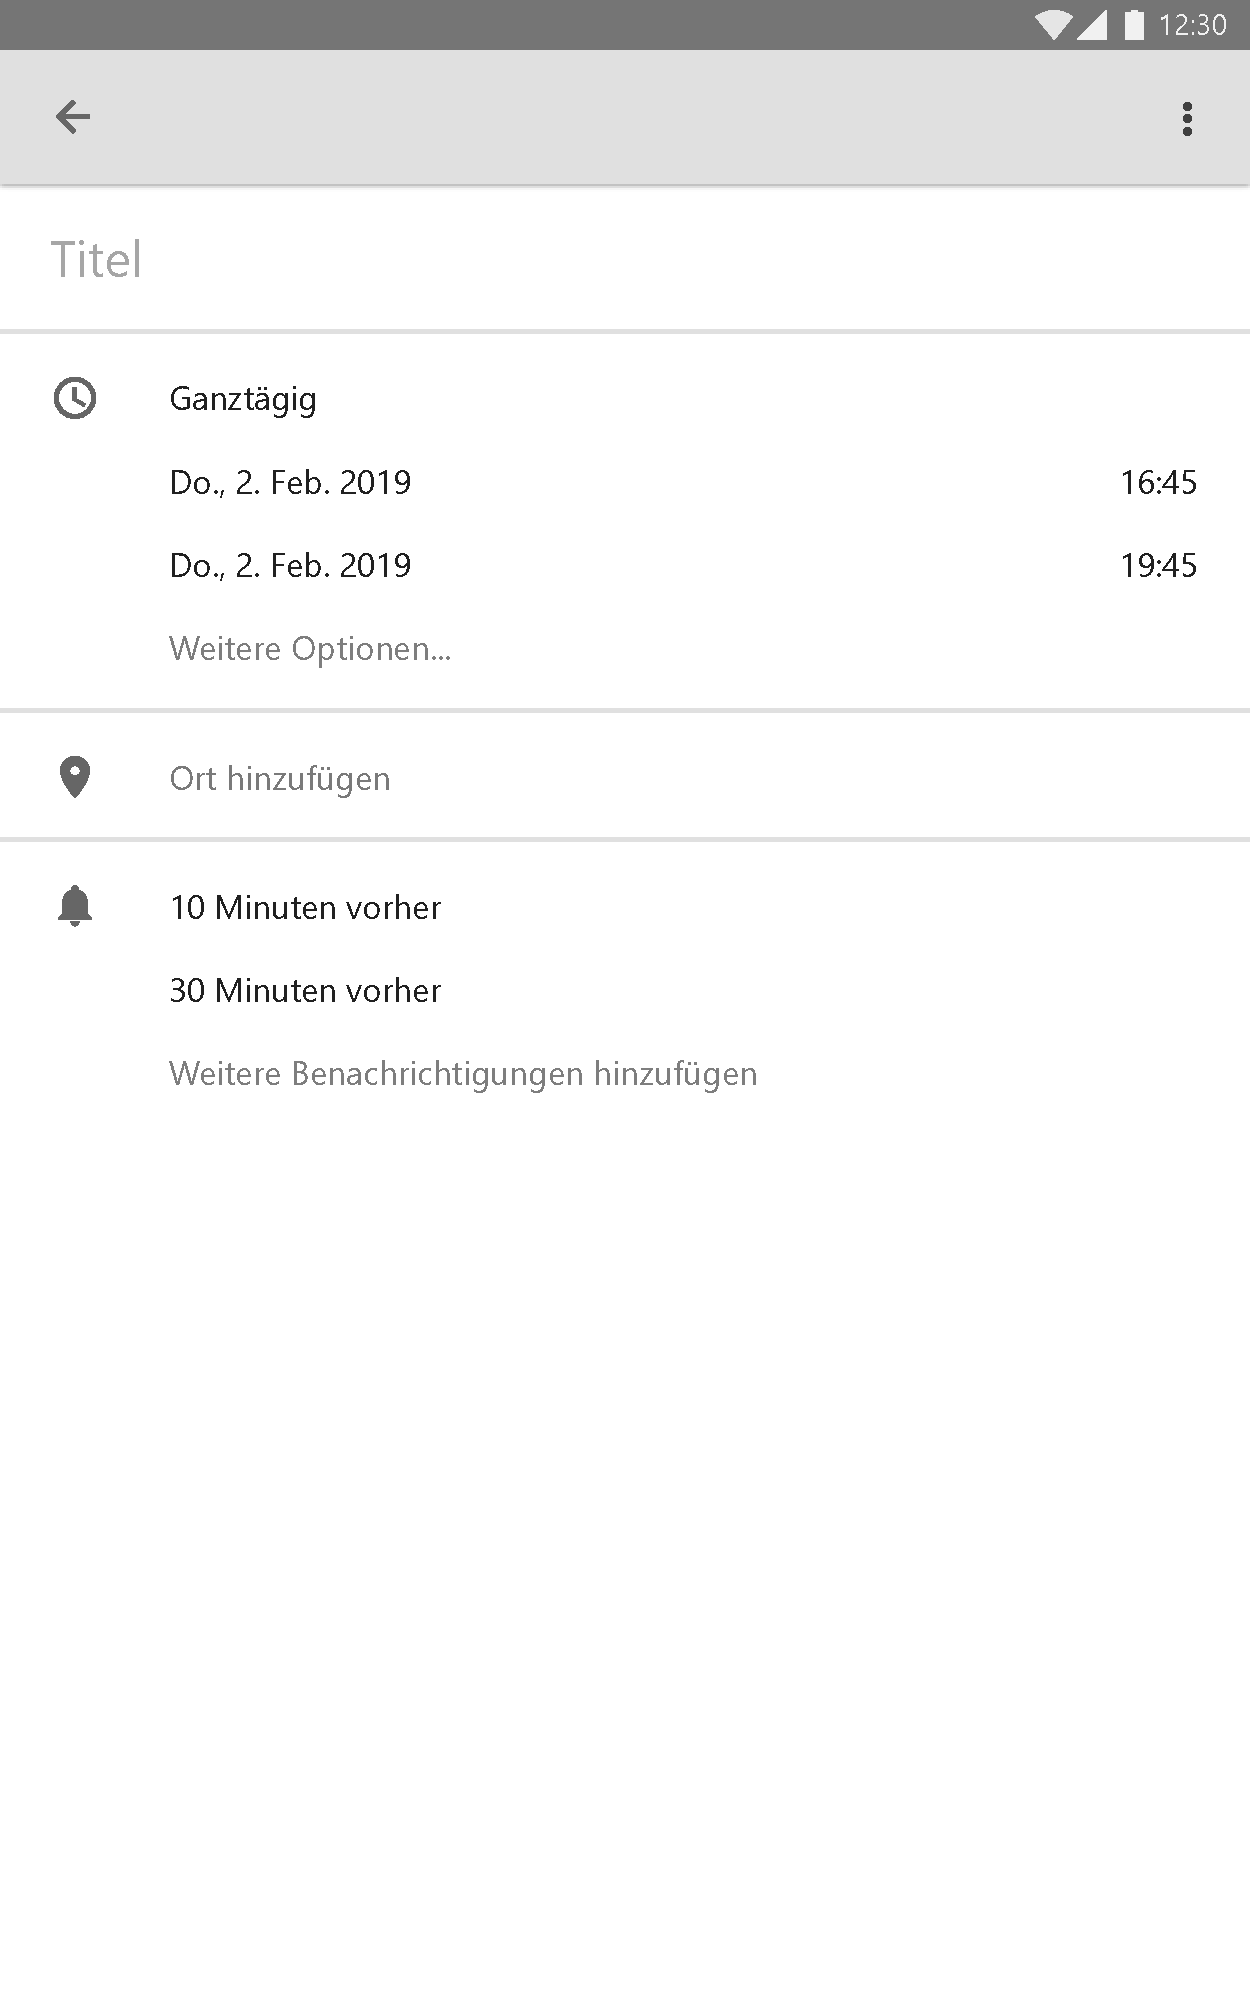
\includegraphics[width=7.25cm]{img/EventActivityNew.pdf}
	\caption{Mockups - Übersicht über ein vorhandenes und ein neues Event}
	\label{img:EventActivity}
\end{figure}

\begin{figure}[H]
	\subsection*{Note Activity - Unsere Notizen}
	\centering
	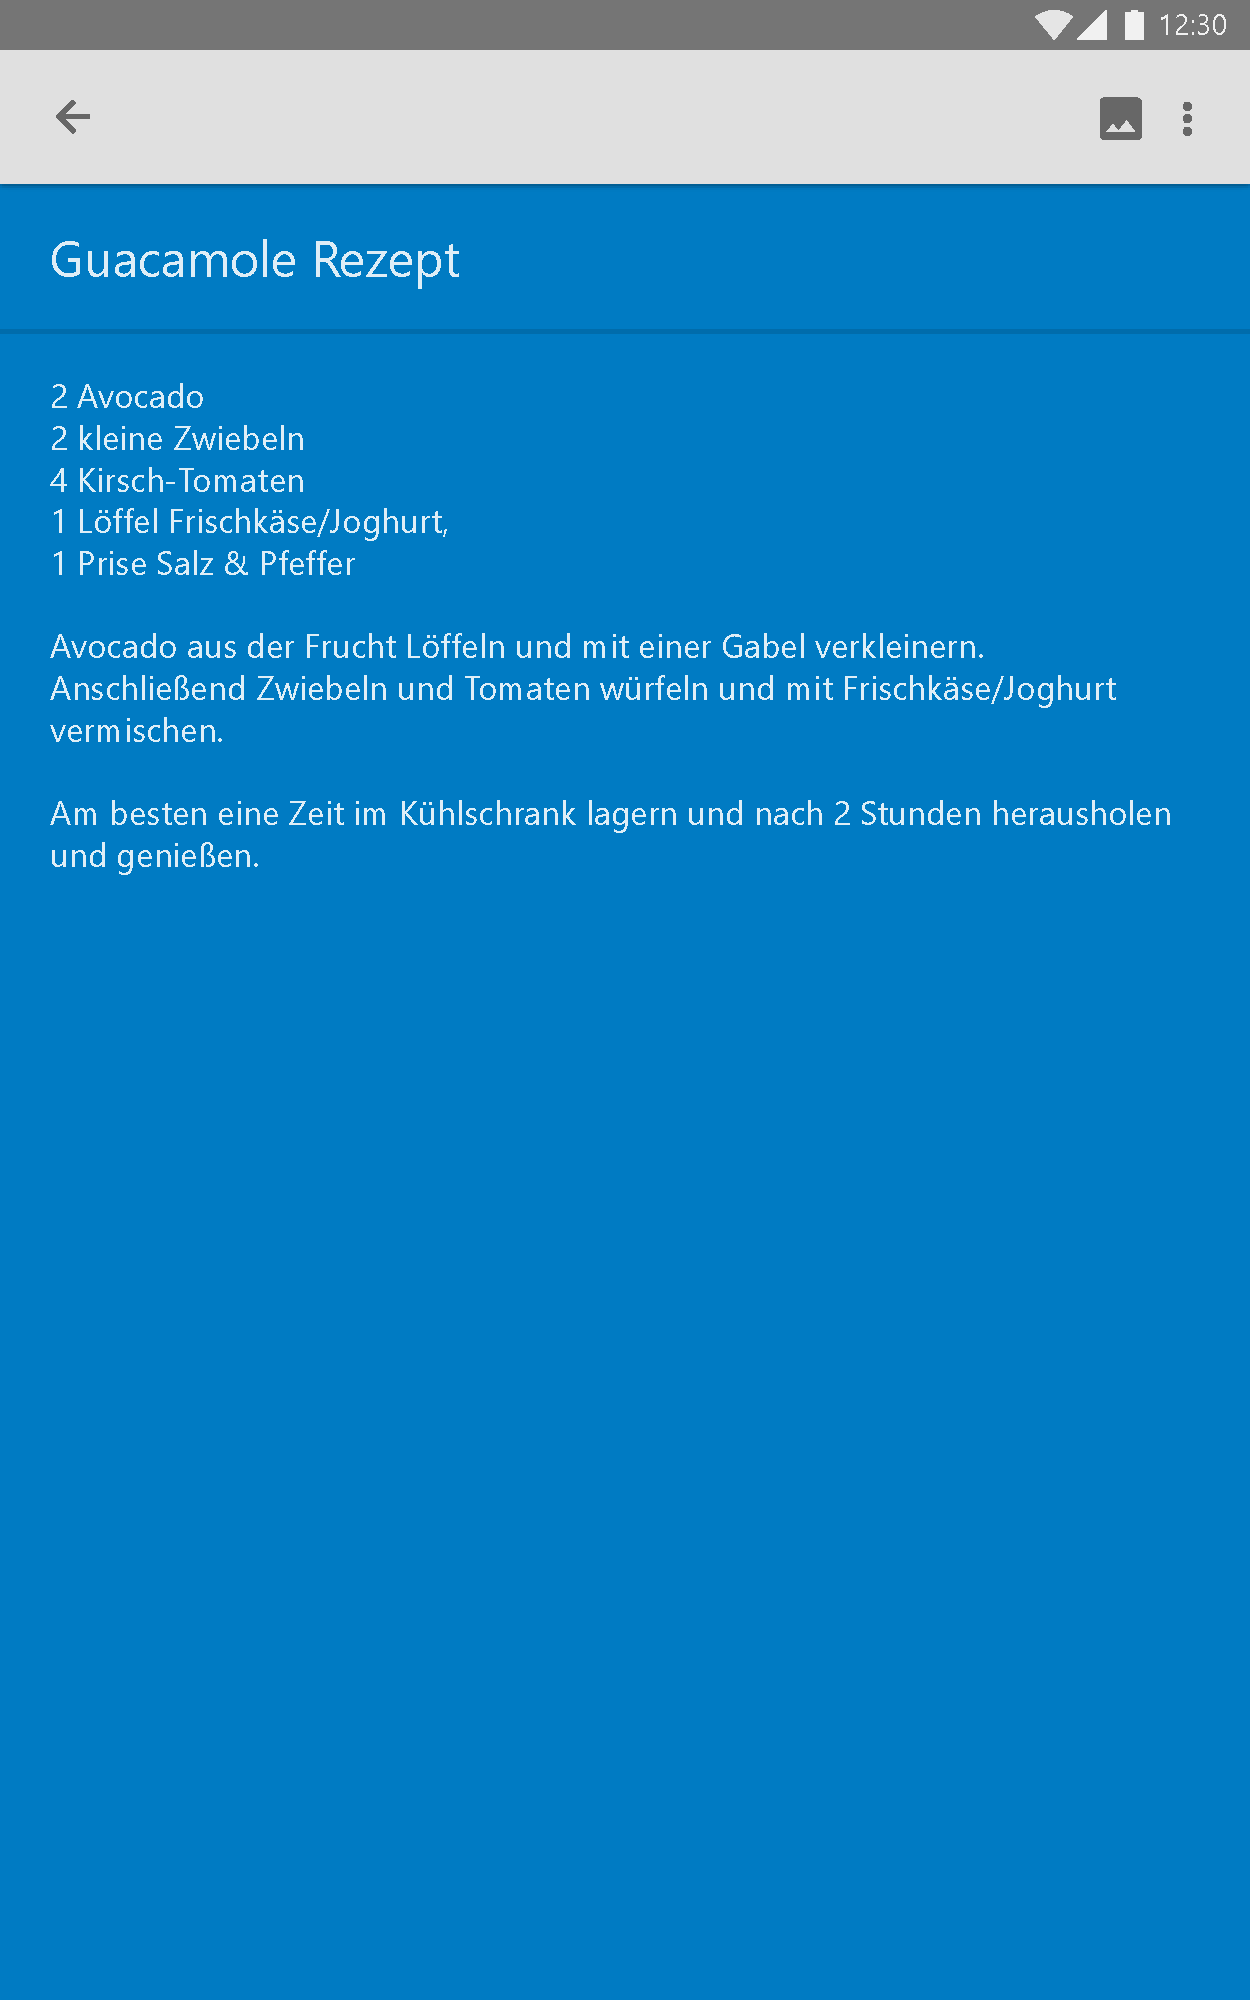
\includegraphics[width=7.25cm]{img/NoteActivity.pdf}
	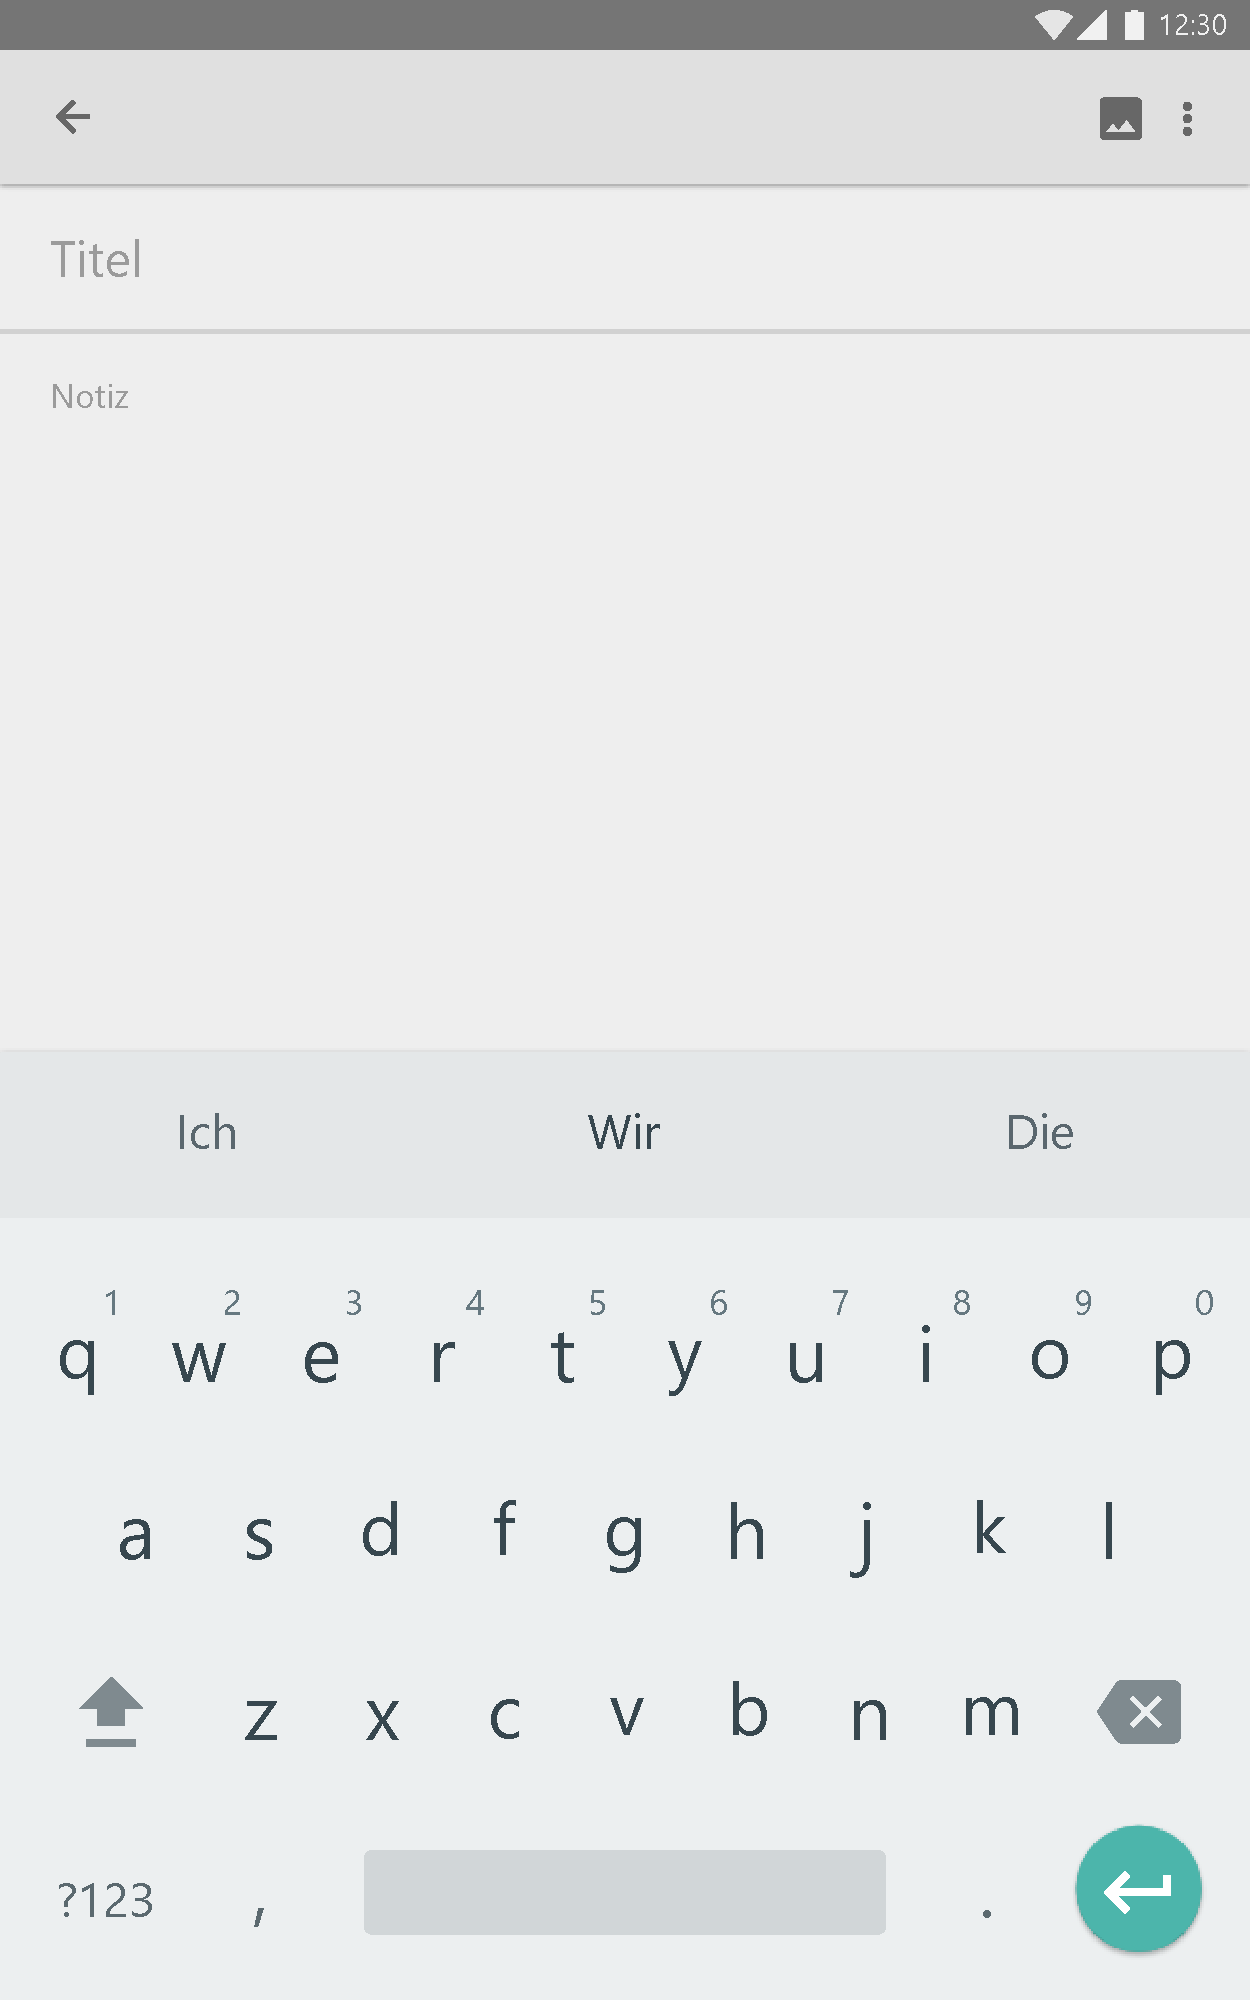
\includegraphics[width=7.25cm]{img/NoteActivityNew.pdf}
	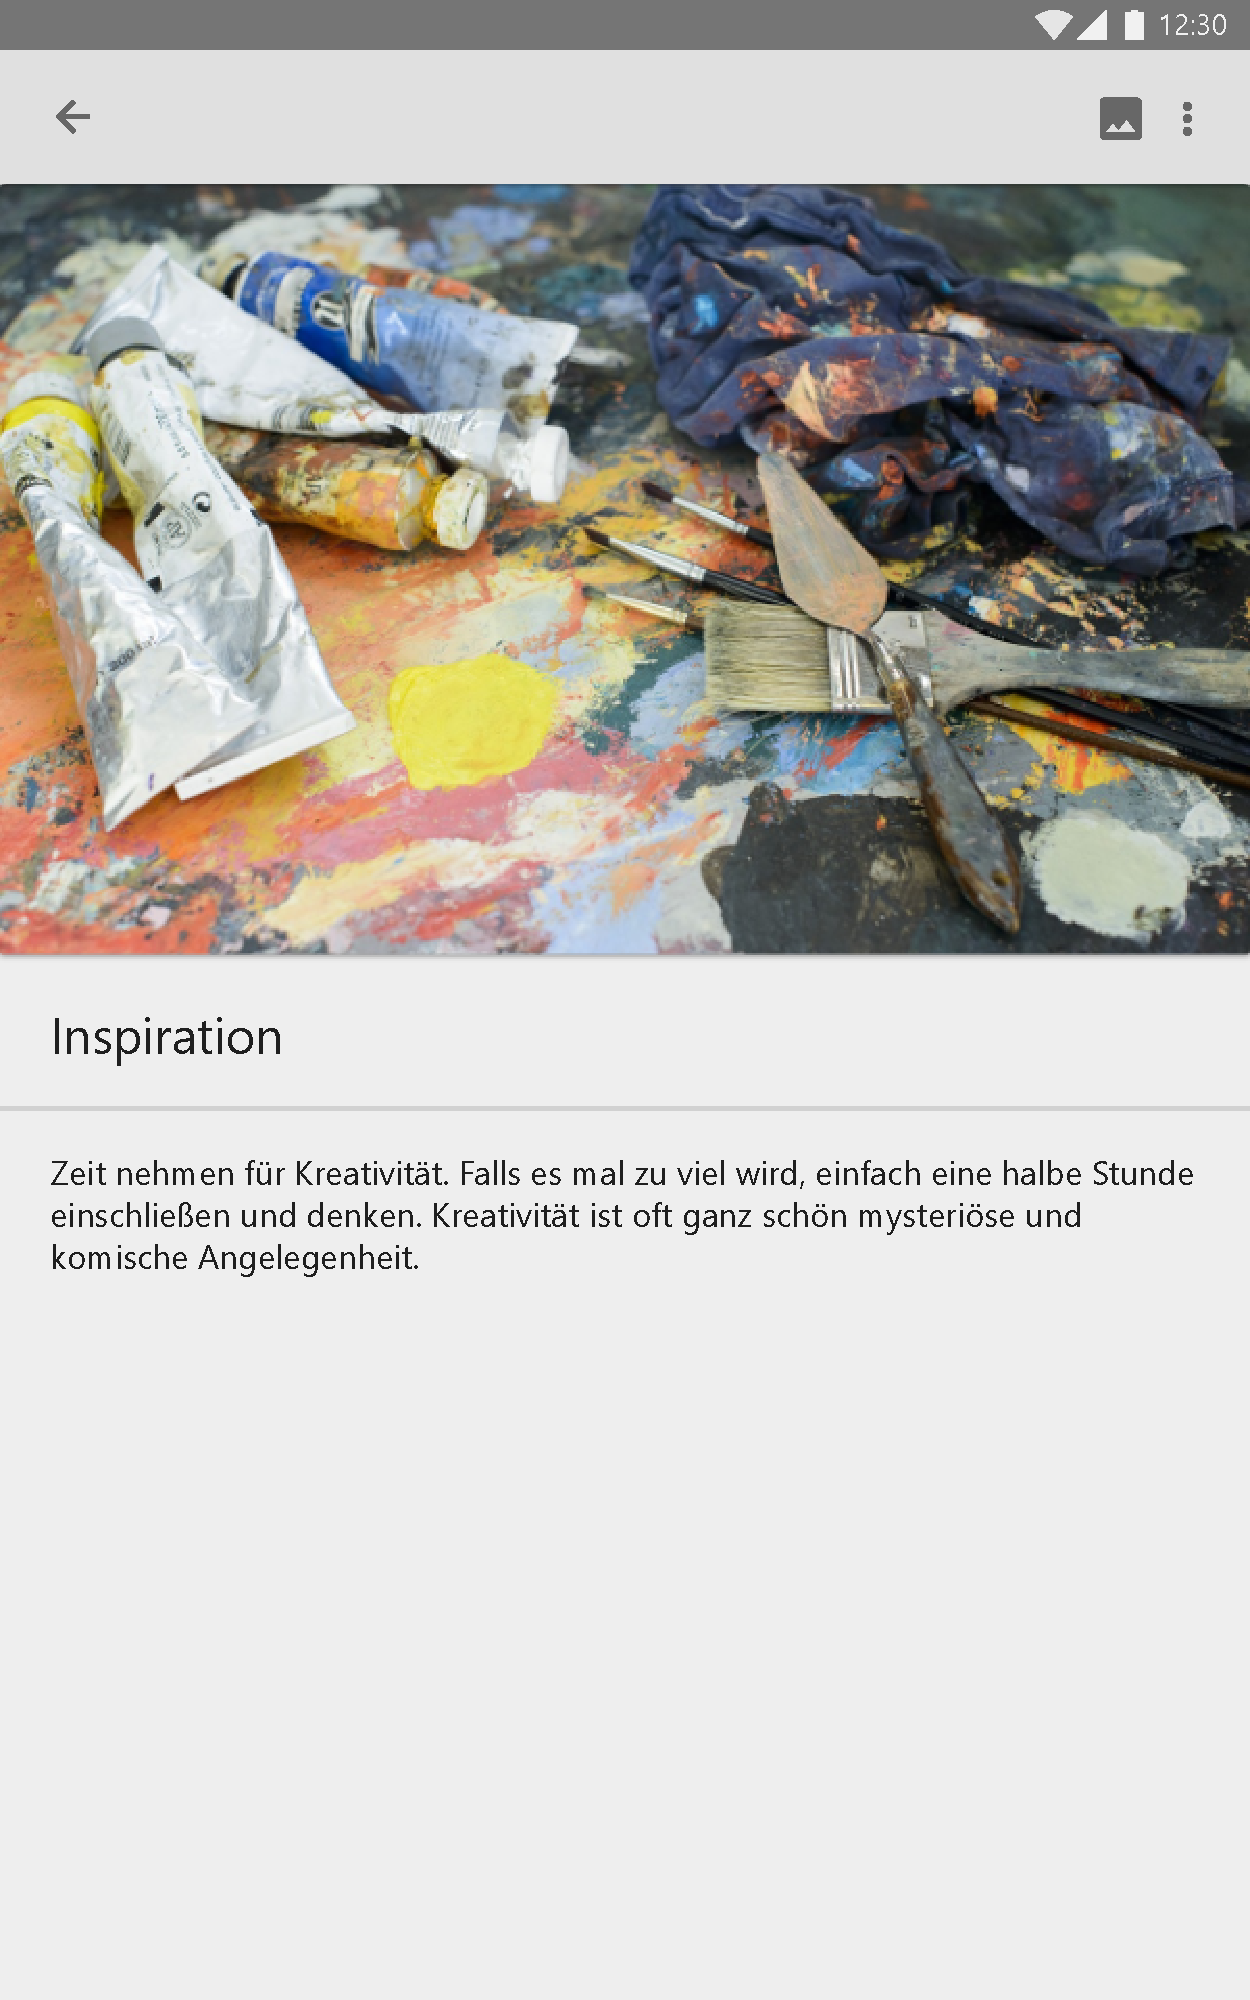
\includegraphics[width=7.25cm]{img/NoteActivityImage.pdf}
	\caption{Mockups - Übersicht über ein vorhandene, eine leere und eine Bild-Notiz}
	\label{img:NoteActivity}
\end{figure}

\begin{figure}[H]
	\subsection*{Todo Activity - Unsere ToDos}
	\centering
	\includegraphics[width=7.25cm]{img/ToDoActivity.pdf}
	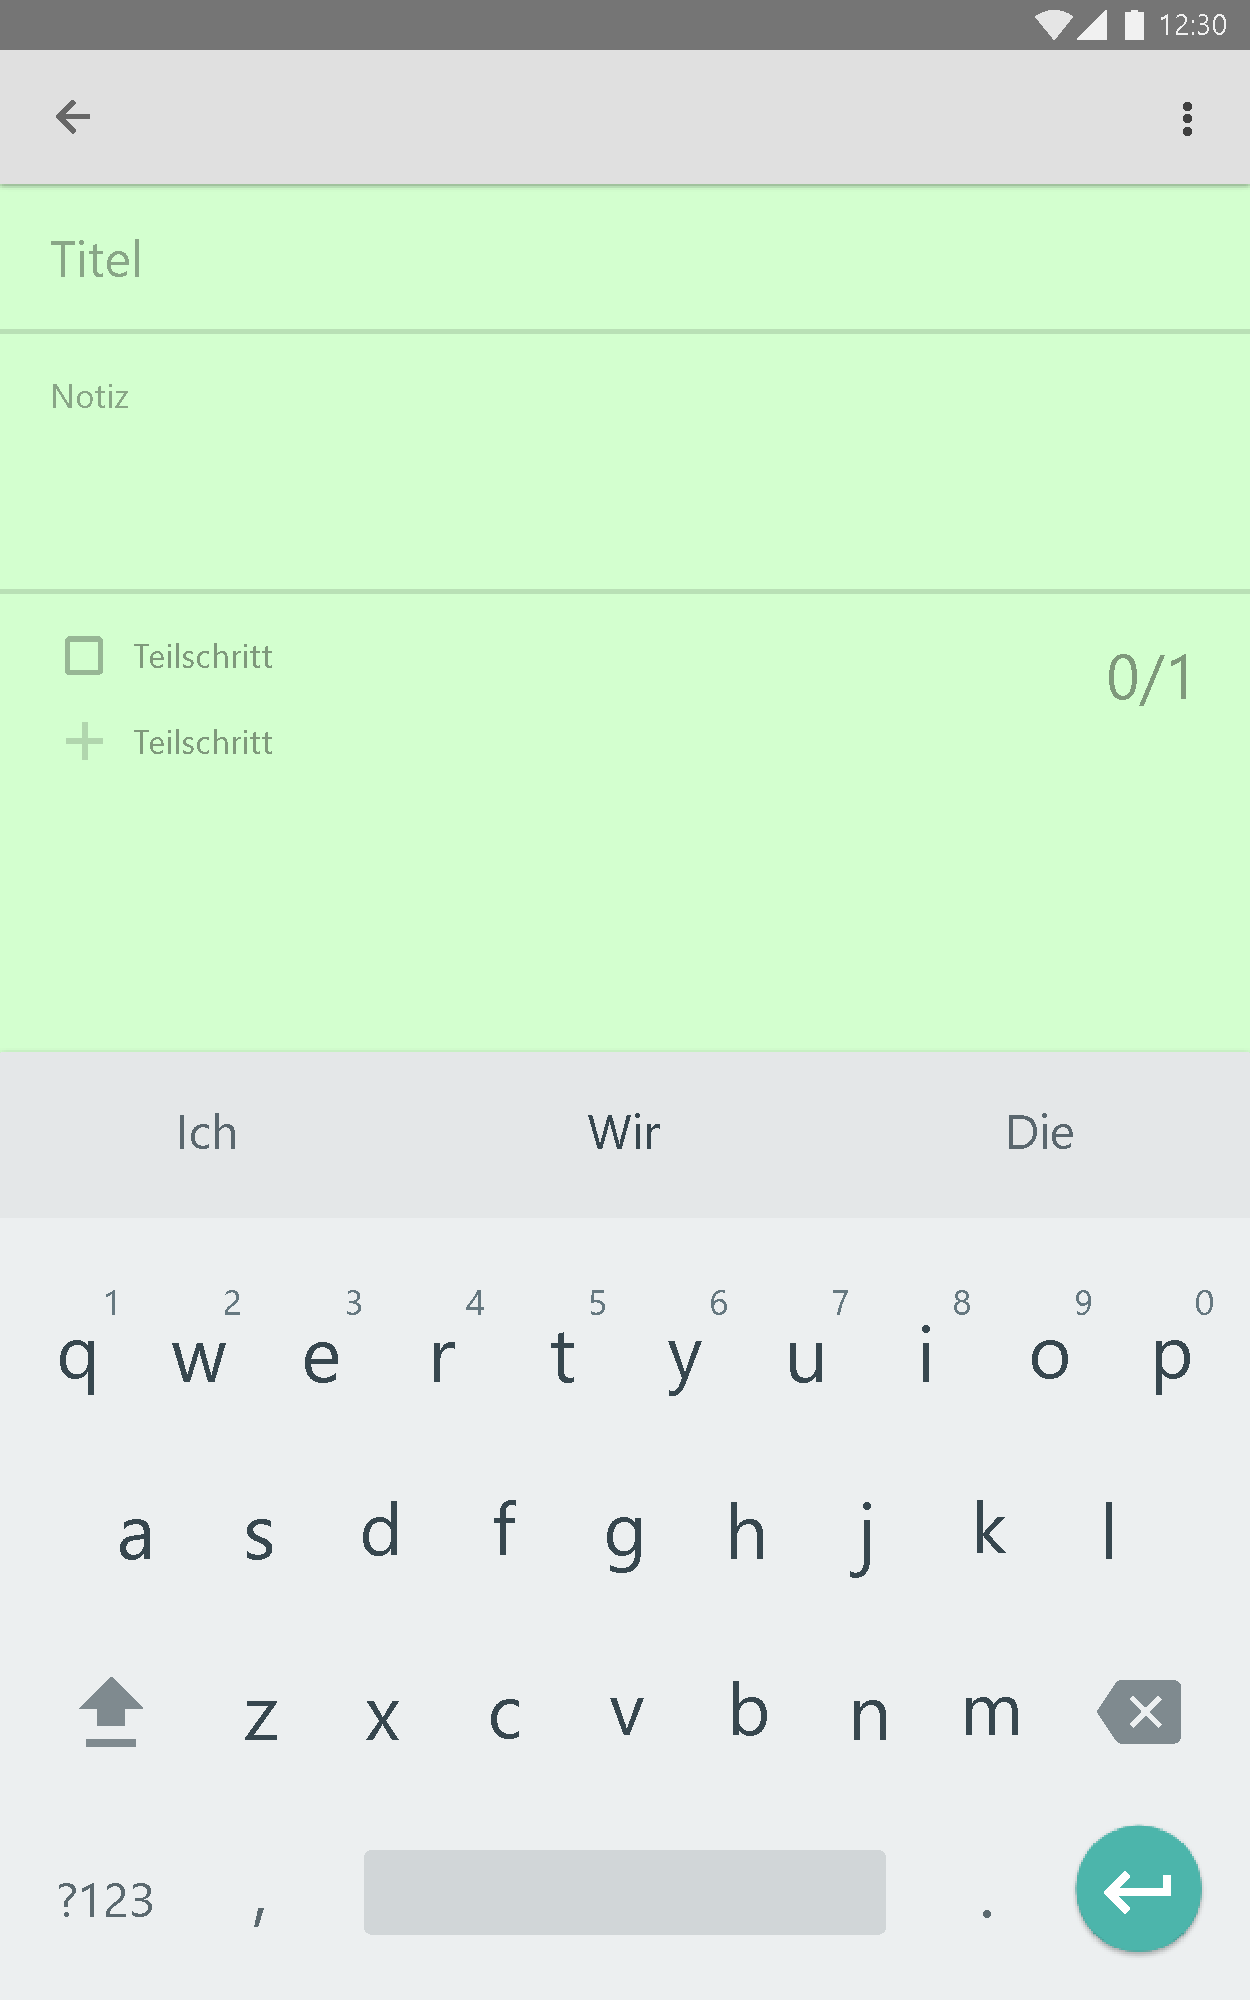
\includegraphics[width=7.25cm]{img/ToDoActivityNew.pdf}
	\caption{Mockups - Übersicht über vorhandene und neue Todos}
	\label{img:ToDoActivity}
\end{figure}

\newpage
\subsubsection{Planung der Datenstruktur und Schnittstellen (Ruthild Gilles)}
%%%%%%%%%
%Ruthild
%%%%%%%%%

Die gewünschte Applikation soll das Managen von Todos, Events und Notes vereinfachen. Anhand der Anforderungen an die Applikation überlegte sich das Datenteam, welche Daten beziehungsweise Informationen in der Datenstruktur der Applikation abgebildet werden sollen. Da sowohl Todo-, Event-, als auch Note-Objekte einheitlich aufgebaut sein sollen, wurde sich dazu entschieden, dass die jeweiligen Klassen von einer TEN-Klasse erben. Alle Todo-, Event- und Note-Objekte benötigen eine ID zu eindeutigen Identifikation des Objektes auf der Datenbank und in der Applikation. Außerdem könnne die Objekte jeweils einen Titel haben. Zudem sollen die verschiedenen Objekte weitere Informationen enthalten. In folgendem Klassendiagramm sind alle geplanten Attribute der Klassen aufgelistet.

\begin{figure}[H]
\centering
\begin{minipage}[t]{1\textwidth} % Breite, z.B. 1\textwidth		
\caption{Klassendiagramm} % Überschrift
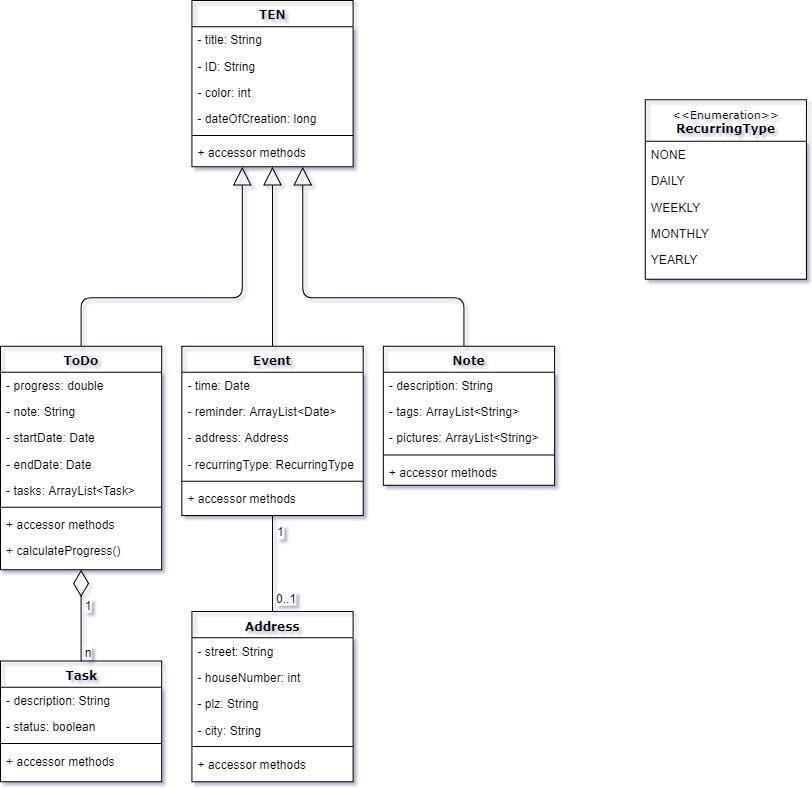
\includegraphics[width=1\textwidth]{img/Klassendiagramm}\\ % Pfad
\source{Erstellt von Joscha Nassenstein} % Quelle
\end{minipage}
\end{figure}

Zusätzlich zu der Struktur der Daten in Form von Klassen mit entsprechenden Attributen wurde ebenfalls die Struktur der Applikation vom Datenteam definiert. Diese ist in nachfolgender Abbildung in einem Systemkontextdiagramm dargestellt.

\begin{figure}[H]
\centering
\begin{minipage}[t]{1\textwidth} % Breite, z.B. 1\textwidth		
\caption{Systemkontextdiagramm} % Überschrift
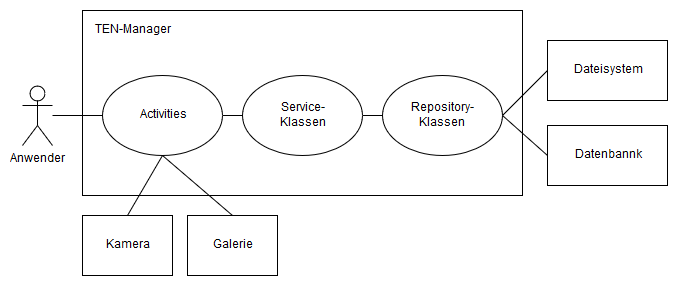
\includegraphics[width=1\textwidth]{img/Systemkontextdiagramm}\\ % Pfad
\source{Erstellt von Ruthild Gilles} % Quelle
\end{minipage}
\end{figure}

Um die Daten auch nach Beendigung der Applikation bei erneutem Starten wieder anzeigen zu können, wurde eine dokumentenbasierte Datenbank an die Applikation angebunden. Auf diese Weise kann eine persistente Datenhaltung erzielt werden. Die einzelnen Activities, welche als Schnittstelle zu den Anwendern dienen, sollen die vom Benutzer eingegebenen Informationen auf der Datenbank speichern können. Dazu sollen Activity-übergreifende Klassen verwendet werden.

Das Datenteam plante die Activity-übergreifenden Klassen und deren Methoden anhand der Anforderungen, der einzelnen Activities. Es sollte möglich sein, einzelne oder auch alle TEN-Objekte von der Datenbank zu erhalten. Auch sollte das Löschen und das Speichern von einzelnen TEN-Objekten möglich sein. Während der Planungsphase wurden hier verschiedene Ansätze in Erwägung gezogen, um diese Anforderungen umzusetzen. Zur Übersichtlichkeit entschied sich das Datenteam letztendlich dafür, einzelne Klassen für jede der vier CRUD-Operationen zu erstellen. Die CRUD-Operationen beinhalten das Erstellen (Create), das Lesen (Read), das Aktualisieren (Update) und das Löschen (Delete) von einzelnen Objekten. Die einzelnen Methoden der CRUD-Klassen sind in folgender Abbildung dargestellt.

\begin{figure}[H]
\centering
\begin{minipage}[t]{1\textwidth} % Breite, z.B. 1\textwidth		
\caption{CRUD-Klassen} % Überschrift
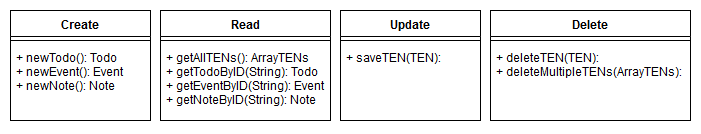
\includegraphics[width=1\textwidth]{img/CRUD-Klassen}\\ % Pfad
\source{Erstellt von Ruthild Gilles} % Quelle
\end{minipage}
\end{figure}

Da der Aufwand für die Umsetzung aller geforderten Anforderungen zu Projektstart lediglich grob geschätzt werden konnte, definierte das Datenteam abgesehen von der Schnittstelle zur Datenbank noch einige weitere Schnittstellen. Die Implementierung dieser weiteren Schnittstellen wurde nicht in den Anforderungen gefordert und würde nur bei genug Zeitüberschuss umgesetzt werden. Zu den weiteren optionalen Schnittstellen gehören das Exportieren von Todos, Events und Notes in die Zwischenablage oder auch in andere Applikationen, die auf dem entsprechenden Endgerät installiert sind. Für ein Event soll es die Möglichkeit geben eine Adresse hinzuzufügen. Hier wäre eine weitere optionale Schnittstelle die Verknüpfung mit Google Maps. Auch könnte eine Schnittstelle zu einer anderen Kalender App implementiert werden, in die ein Event exportiert werden könnte.

\newpage

\subsubsection{Planung der Activities und Layouts (Florian Rath)}
%%%%%%%%%
%Florian
%%%%%%%%%

Hier den Text einfach hin kopieren.

\subsubsection{Planung der Navigation zwischen den Activities (Yannick Rüttgers)}
%%%%%%%%%
%Yannick
%%%%%%%%%

Hier den Text einfach hin kopieren.

\subsection{Geplante Aufgabenverteilung im Team (Fabia Schmid)}
%%%%%%%%%
%Fabia
%%%%%%%%%

Hier den Text einfach hin kopieren.

%%%%%%%%%%%%%%%%%%%%%%%%%%%%%%%%%%%%%%%%%%%%%%%%%%%%%
%Als Beispiel
%Bitte noch entfernen:

So kann man Abbildungen einfügen:

\begin{figure}[H]
\centering
\begin{minipage}[t]{1\textwidth} % Breite, z.B. 1\textwidth		
\caption{Abbildungsbeschriftung} % Überschrift

\includegraphics[width=1\textwidth]{img/fhdw}\\ % Pfad
\source{\url{http://dominique-fleury.com/?p=302}} % Quelle
\end{minipage}
\end{figure}

